\chapter{Setting the Stage}  
\label{chap:prologue} 

Let's first get an overview of the topic and the nature of this book.
Keep in mind, this is just an overview; many questions should come to
your mind, hopefully whetting your appetite for the succeeding chapters!

In this chapter, we will mainly describe \textit{collaborative
filtering}, one of several common approaches to recommender systems
(RTSs). 

\section{What Are Recommender Systems?}

What is an RS?  We're all familiar with the obvious ones---Amazon
suggesting books for us to buy, Twitter suggesting whom we may wish to
follow, even OK Cupid suggesting potential dates. 

But many applications are less obvious.  The University of Minnesota,
for instance, has developed an RS to aid its students in selection of
courses.  The tool not only predicts whether a student would like a
certain course, but also even predicts the grade she would get!

In discussing RS systems, we use the terms \textit{users} and
\textit{items}, with the numerical outcome being
termed the \textit{rating}.  In the famous MovieLens dataset, which
we'll use a lot, users provide their ratings of films.

Systems that combine user and item data as above are said to perform
\textit{collaborative filtering}.  The first part of this book will
focus on this type of RS.  \textit{Content-based} RS systems work by
learning a user's tastes, say by text analysis.

Ratings can be on an ordinal scale, e.g.\ 1-5 in the movie case.  Or 
they can be binary, such as a user clicking a Like symbol in Twitter, 1 for a
click, 0 for no click.

But ratings in RSs are much more than just the question, ``How much do
you like it?''  The Minnesota grade prediction example above is an
instance of this.

In another example, we may wish to try to predict bad reactions to
prescription drugs among patients in a medical organization.  Here the
user is a patient, the item is a drug, and the rating may be 1 for
reaction, 0 if not.  

More generally, any setting suitable for what in statistics is called
a \textit{crossed heirachical model} fits into RS.  The word
\textit{crossed} here means that each user is paired with multiple
items, and vice versa.  The hierarchy refers to the fact that we can
group users within items or vice versa.  There would be two levels of
hierarchy here, but there could be more.  

Say we are looking at elementary school students rating story books.  We
could add more levels to the analysis, e.g. kids within schools within
school districts.  It could be, for instance, that kids in different
schools like different books, and we should take that into account in
our analysis.  The results may help a school select textbooks that are
especially motivational for their students.

Note that in RS data, most users have not rated most items.  If we form
a matrix of ratings, with rows representing users and columns indicating
items, most of the elements of the matrix will be unknown.  We are
trying to predict the missing values.  Note carefully that these are not
the same as 0s.

\section{The ``Hello World'' of RS:  MovieLens}

This dataset is the standard introduction to RSs, and indeed is a
standard example in RS research papers.  It's available from the
GroupLens project at the University of Minnesota, \url{grouplens.org}.
In this book, we will mainly use the 100K version, which contains
100,000 rates in the format

\begin{lstlisting}
userID  movieID  rating1to5  timestamp
\end{lstlisting}

Let's take a look:

\begin{lstlisting}
> ml100 <- read.csv('ml100k.data',header=FALSE,sep='\t')
> head(ml100)
   V1  V2 V3        V4
1 196 242  3 881250949
2 186 302  3 891717742
3  22 377  1 878887116
4 244  51  2 880606923
5 166 346  1 886397596
6 298 474  4 884182806
\end{lstlisting}

(Note that the data comes in TAB-separated fields.)

So for instance user 22 rated movie 377 as 1.  Let's explore some more:

\begin{lstlisting}
> length(unique(ml100$V1))
[1] 943
> length(unique(ml100$V2))
[1] 1682
> table(ml100$V3)

    1     2     3     4     5 
 6110 11370 27145 34174 21201 
\end{lstlisting}

So there were 943 users and 1682 films.  Users seemed to be pretty
liberal in their ratings, with the most popular rating being a 4.

We can break that down by user:

\begin{lstlisting}
> tmp <- tapply(ml100$V3,ml100$V1,mean)
> tmp[22]
      22 
3.351562 
> hist(tmp)
\end{lstlisting}

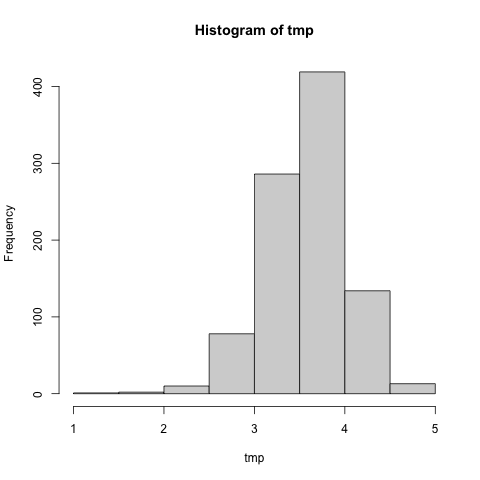
\includegraphics[width=4.5in]{Images/Ch1HistMeanRatings.png}

So for instance user 22 gave an average rating of about 3.35 to the ones
he/she rated.  And how many films was that?

\begin{lstlisting}
> tmp <- tapply(ml100$V3,ml100$V1,length)
> tmp[22]
 22 
128 
\end{lstlisting}

Did user 22 rate movie 88?

\begin{lstlisting}
> ml100[ml100$V1 == 22 & ml100$V2 == 88,]
[1] V1 V2 V3 V4
<0 rows> (or 0-length row.names)
\end{lstlisting}

No.  And that is the essence of RS:  How can we predict what rating user
22 would give to that movie?


\section{How Is It Done?}

Putting aside possible privacy issues that arise in some of the above RS
applications,\footnote{I used to be mildy
troubled by Amazon's suggestions, but with the general demise of
browsable bricks-and-mortar bookstores, I now tend to view it as ``a
feature rather than a bug.''} we ask here, How do they do this?  In this
prologue, we'll discuss a few of the major methods for collaborative
filtering (CF)..

\subsection{Nearest-Neighbor Methods}

This is probably the oldest class of RS methodology, still popular
today.  It can be explained very simply.

Say there is a movie spoofing superheroes called \textit{Batman Goes
Batty} (BGB).  Maria hasn't seen it, and wonders whether she would like
it.  To form a predicted rating for her, we could search in our dataset
for the $k$ users most similar to Maria in movie ratings and who have
rated BGB.  We would then average their ratings in order to derive a
predicted rating of BGB for Maria.  We'll treat the issues of choosing
the value of $k$ and defining ``similar'' later, but this is the
overview.

In general, methods like this are called k-NN methods,
for ``k-nearest neighbor.''  (We'll shorten it to kNN.)
Actually, kNN was one of the earliest methods in machine learning in
general.

\subsection{Latent Factor Approach:  Matrix Factorization}
\label{mf}

This one is less intuitive, but is probably the most popular CF methods.

Let $A$ denote the matrix of ratings described earlier, with $A_{ij}$
denoting the rating user $i$ gives to item $j$.  Keep in mind, as noted,
that most of the entries in $A$ are unknown; following R convention,
we'll refer to them as NA, the R-language notation for missing values.  
So for our movie example above, \lstinline{bf{A[22,377] = 1} and
\lstinline{A[22,88] = NA}.

Matrix factorization (MF) methods then estimate all of $A$ as follows.
Let $r$ and $s$ denote the numbers of rows and colums of $A$,
respectively.  In our data above, for example, $r = 943$ and $s = 1682$.
The idea is to find a \textit{low-rank approximation} to $A$:  Using our
known ratings, we find matrices $W$ and $H$, of dimensions $r \times m$
and $m \times s$, each of rank $m$, such that 

\begin{equation}
A \approx WH
\end{equation}

Typically $m << \min(r,s)$.  Software libraries typically take 10 as the
default.

We will review the concept of matrix rank later, but for now the key is
that $W$ and $H$ are \underline{known} matrices, no NA values.  Thus we
can form the product $WH$, thus obtaining estimates for all the missing
elements of $A$.

For our example above, our predicted value for user 22's rating of
moveie 88 would be

\begin{equation}
(WH)_{22,88}
\end{equation}

\subsection{Latent Factor Approach: Statistical Models}

As noted, collaborative-filtering RS applications form a special case of
crossed random-effects models, a statistical methodology.  In that way,
a useful model for $Y_{ij}$, the rating user $i$ gives item $j$, is

\begin{equation}
Y_{ij} = \mu + \alpha_i + \beta_j + \epsilon_{ij}
\end{equation}

a sum of an overall mean, an effect for user $i$, an effect for item
$j$, and an ``all other effects'' term (often called the ``error
term'').

In the MovieLens setting, $\mu$ would be the mean rating given to all
movies (in the ``population'' of all movies, past, present and future),
$\alpha_i$ would be a measure of the tendency of user $i$ to give
ratings more liberal or harsher than the average user, and $\beta_j$
would a measure of the popularity of movie $j$, relative to the average
movie.

What assumptions are made here?  First, $\mu$ is a fixed but unknown
constant to be estimated.  As to $\alpha_i$ and $\beta_j$, one could on
the one hand treat them as fixed constants to be estimated.  On the
other hand, there are some advantages to treating them as random
variables, we will be seen in Chapter \ref{chap:mixed}.

It is customary to use the ``hat'' notation $\widehat{}$ to mean
``estimate of.''  After finding estimates of the above model quantities
from our data, our predicted value for user 22 and movie 88 would then
be

\begin{equation}
\widehat{A}[22,88] = \widehat{\mu} + \widehat{\alpha}_{22} + 
\widehat{\beta}_{88}
\end{equation}

\subsubsection{Comparison}

Why so many methods?  There is no perfect solution, and each has
advantagages and disadvantages.

First, note that in the kNN and MF methods, the user must choose the
value of a design parameter.  In kNN, we must choose $k$, the number of
nearest neighbors, and while in MF, we must choose $m$, the rank.

Parameters such as $k$ and $m$ are known as \textit{tuning parameters}
in statistics and \textit{hyperparameters} in machine learning (ML).
Many ML methods have multiple hyperparameters, sometimes 10 or more.
This can be quite a drawback, as choosing their values is quite
difficult.  By contrast, the statistical model described above has no
tuning parameters.

A problem with both MF and the statistical models is that one is limited
to prediction only of ratings for users and items that are already in
our dataset.  We could not predict a new user, for instance, without
recomputing an updated fit.  With kNN, there is no such restriction.

\section{Tuning Parameters}

The reader is likely familiar with histograms.  Recall that the analyst
must choose a bin width.  Here there is a tradeoff:

\begin{itemize}

\item If the width is too small, some bins will have no data points, or
very few.  This will produce a very choppy appearance.

\item But it's also bad to have too large a width.  In the extreme, we
have bins so wide that we have just one of them, totally uninformative.

\end{itemize} 

The bin width is called a \textit{tuning parameter} or a
\textit{hyperparameter}.  Most machine learning algorithms, including
most in recommender systems, have several tuning parameters.  Choosing
the values of those parameters is not easy, but there are methods for
it.

\textbf{Important note:} Think of datasets A and B, similar but A having
only 25 data points and B having 500.  Then the problem of empty or
nearly-empty bins is much less of an issue.  In other words, we can
afford to make the bin width smaller if we have dataset B, thus getting
a more detailed picture.

\section{Covariates/Side Information}

In predicting the rating for a given (user,item) pair, we may for
example have demographic information on the user, such as age and
gender.  Incorporating such information --- called \textit{covariates}
in statistics and \textit{side information} in machine learning --- may
enhance our predictive ability, especially if this user has not rated
many items to date.

\section{Prerequisites}

What is background is needed for this book?

\begin{itemize}

\item A calculus-based probability course.

\item Some facility in programming.  

\item Good mathematical intuition.

\end{itemize} 

We will be using the R programming language.  No prior experience with R
is assumed.  A Quickstart in R is available in Appendix
\ref{chap:rquickstart}.

We will also use some machine learning techniques, but no prior
background is assumed.

\section{Software}

A number of libraries are available for RS methods.  We will use the R
package \textbf{rectools}, available in my GitHub repo,
\textbf{github.com/matloff}.

\section{What You Should Gain from This Book}

\begin{itemize}

\item A solid understanding of RS fundamentals:  You'll be able to build
simple but effective RS systems, and will be able to read books and
research on advanced RS methods.

\item Greatly enhanced understanding of the basics of
probability/statistics, machine learning and linear algebra.

\end{itemize} 

